\documentclass{standalone}
\usepackage[T1]{fontenc}
\usepackage[utf8]{inputenc}
\usepackage{pgf,tikz}
\usetikzlibrary{calc}
\usepackage{pgfplots}
\usepackage[amssymb]{SIunits}


\begin{document}
  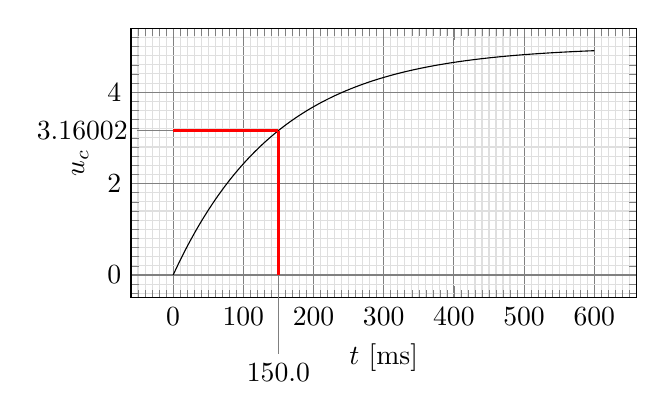
\begin{tikzpicture}[node distance=20mm]
     \def\Gain{5}
     \pgfmathsetmacro{\RR}{1} % in kOhm
     \pgfmathsetmacro{\CC}{150} % in micro C 
     \pgfmathsetmacro{\Timeconst}{(\RR * \CC)} % in ms
     \pgfmathsetmacro{\xmax}{\Timeconst*4}
     \pgfmathsetmacro{\ucattc}{\Gain*0.632}

     %\node {\large \Timeconst};

     \begin{axis} [
       width=8cm,
       height=5cm,
       xlabel={$t$ [ms]},
       ylabel={$u_c$},
       grid = both,
       minor tick num=9,
       minor grid style={gray!25},
       major grid style={black!50},
       clip=false,
       ]
       
       \addplot+[no marks, black, domain=0:\xmax, samples=200 ] { \Gain * (1 - exp(-x/\Timeconst)};

       \draw[thick, red] (axis cs: 0, \ucattc) to (axis cs: \Timeconst, \ucattc);
       \draw[thick, red] (axis cs: \Timeconst, \ucattc) to (axis cs: \Timeconst, 0);
       \node[coordinate, pin=180:{\ucattc}] at (axis cs: 0, \ucattc) {};
       \node[coordinate, pin={[pin distance=10mm] -90:{\Timeconst}}] at (axis cs: \Timeconst, 0) {};
     \end{axis}
   \end{tikzpicture}
 \end{document}
 